% Preamble
\documentclass{article}


% Packages
\usepackage{amsmath}  % Adanced math typesetting
\usepackage{amsfonts}  % Adanced math typesetting
\usepackage{xcolor}
% \usepackage[uft9]{inputenc}  % Unicode support
% \usepackage[ngerman]{babel}  % change hyphenation rules
% \usepackage{hyperref}  % Add link to doc
\usepackage{graphicx}  % Add pictures to your doc
% \usepackage{listings}  % Source code formating and highlighting
\usepackage{amsthm}

\newtheorem{definition}{Definition}
\newtheorem{theorem}{Theorem}



\begin{document}

\author{Sean Jennings}
\title{System Identification Notes}
\date{\today{}}
\maketitle{}
\tableofcontents{}
\newpage{}


\section{Digital Signals Background: Convolution}

We'll use analogies to audio processing for this section.
In simplest terms, convolution consists of three operations:
\begin{enumerate}
    \item{Delaying a signal by some fixed number of samples}
    \item{Applying a gain to the delayed signal}
    \item{Mixing the delayed and gained signal with the original}
\end{enumerate}

\subsection{Example: Delay and Mix}
First, we will consider the case where no gain is applied. Take the
output signal:
\begin{align}
    y[n] = x[n]+ x[n - k]
\end{align}
Taking a square wave as input, Figure ~\ref{fig:mix_and_delay} shows the output for k=2
\begin{figure}
    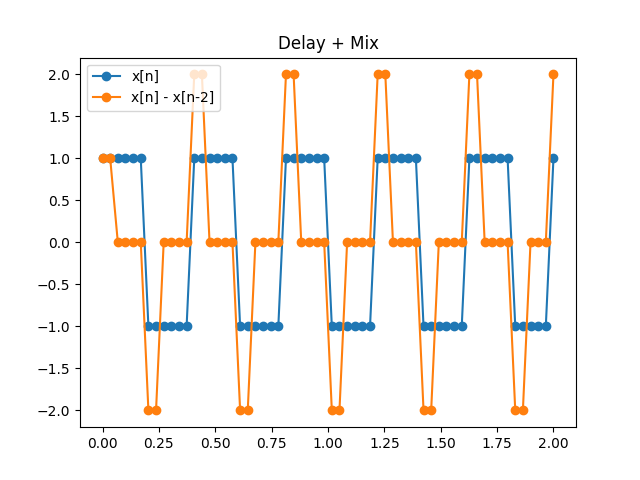
\includegraphics[width=\linewidth]{conv_plots/Delay + Mix.png}
    \caption{x[n] - x[n-2] for square wave input}
    \label{fig:mix_and_delay}
\end{figure}

\subsection{Definitions}
A {\it filter} is some function $g$ which transforms a signal:
\begin{equation}
    y = g(x)
\end{equation}

A {\it convolutional filter} is a function which applies convolution to the input signal.
Given an input signal ${x[n]}$ and a convolutional filter $h[k]$ of length $K$,
the convolution $h * x$ is computed by:
\begin{equation}
    y[n] = \sum_{k=0}^K h[k] * x[n -k]
\end{equation}

\subsection{Example: Moving window average}
A moving average of a signal can be computed via a convolution.
The convolutional filter
\begin{equation}
    h = \bigl[
        \underbrace{
            1/m \quad 1/m \quad \cdots \quad 1/m
        }_{\text{$m$ elements}}
    \bigr]
\end{equation}

will average the last $m$ samples with even weights. An example is shown in Figure
~\ref{fig:moving_average}.

\begin{figure}
    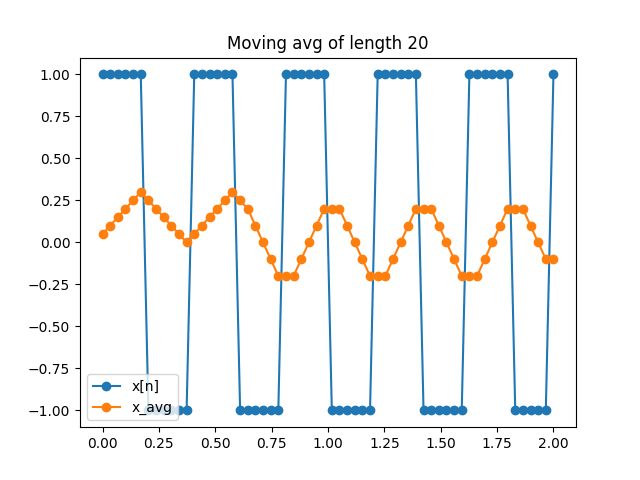
\includegraphics{conv_plots/Moving avg of length 20.png}
    \caption{A square wave x[n] with a moving average convolution (m=20) applied}
    \label{fig:moving_average}
\end{figure}

\subsection{Impulse response}
An impulse is a theoretical construct, the idealized signal consisting of a single
$1$ followed by infinitely many zeros:
\begin{align}
    x_| &= [1 \quad 0 \quad 0 \quad 0 \quad \cdot] \\
    x_|[n] &= \left\{
            \begin{array}{ll}
                1 & \quad n=0 \\
                0 & \quad n\neq0
            \end{array}
        \right.
\end{align}



The {\it impulse response} of a filter $g$ is the output signal $y$ that is produced
when applying $g$ to an impulse $x_|$.

We will look specifically at a filter operation that is a convolution between
an input signal $x$ and a fixed length sequence $h$. We may then ask,
what is the impulse response of a convolutional filter? By the
definition of convolutional filters:
\begin{equation}
    y[n] = \sum_{k=0}^K h[k] * x_|[n - k]
\end{equation}

Since $x_| = 0 \ \forall  n \neq k$
\begin{align}
    y[n] &= h[n] * x_|[0] \\
    y[n] &= h[n]
\end{align}

So the impulse response of a convolutional filter is equal to the sequence $h$ itself!
In other words, the impulse response is enough to fully characterize a convolutional
filter.

\subsection{Convolutional modes}
The convolution $y = x * h$ depends on {\it negative sample indices} for 
indices where $n < k < K$. This is generally handled by assuming
$x[n] = 0 \ \forall n<k$. This can also be thought of as prepending (padding) the
input sample with zeros, thus ensuring that convolution is well-defined for
these indices. Therefore the first $K - 1$ samples of $y$ will depend on the 
padding.

Since it may or may not be appropriate to use the output which depends on
padded values, there are different {\it modes} which define some combination of
trimming and padding the inputs and outputs. Note: this does not affect the nature
of how convolution itself works.

We will assume $x$ and $h$ have $N$ and $K$ samples, respectively, and for
convenience, that $K < N$, although this is not strictly necessary.

\subsubsection{Full Mode}
Full mode is attained by padding the input by $K - 1$ zeros both and the beginning
and end. This results in an output of length $N + K - 1$. For intuition, these
can be thought of as {\it warming up} and {\it ringing out} phases.

\subsubsection{Valid Mode}
Valid mode eliminates outputs that depend on the padding. Therefore, the output
will have length of $N - K + 1$.

\subsubsection{Same Mode}
Same mode produces an output that is the same length as the input. This is typically
done by extracting the middle of the output, so that the first and last $K/2$ samples
depend on padding.

It can also be trimmed from the beginning or end of the full mode output, so that
either warmup or ring out effects are included.

\begin{table}[h!]
    \begin{center}
        \caption{Convolutional Modes}
        \label{tab:conv_modes}
        \begin{tabular}{c|c|c}
            \textbf{Mode} & \textbf{length} & \textbf{slice} \\
            \hline \\
            Full & N + K - 1 & 0 : N + K - 1 \\
            Valid & N - K + 1 & K : N \\
            Same (left) & N & 0 : N \\
            Same (center) & N & (K - 1)//2 : N + (K - 1)//2 \\
            Same (right) & N & K - 1: N + K - 1 \\
        \end{tabular}
    \end{center}
\end{table}

\subsection{Properties of convolutions}
Convolution can be thought of as a kind of multiplication between signals. 
We will thus explore the properties of convolutions:

\subsubsection{Communicative}

If $x$ is a signal and $h$ is an impulse reponse, then
\begin{equation}
    \textcolor{blue}{x} * \textcolor{red}{h} = \textcolor{red}{h} * \textcolor{blue}{x}
\end{equation}

This implies that there is no difference between {\it signals} and {\it filters}.

\subsubsection{Associative}

Convolution also has the associative property, meaning it does not matter which
order operations are applied.
If $x$ is a signal and $h$ and $g$ are impulse responses
\begin{equation}
    \textcolor{red}{g} * (h * x) = (\textcolor{red}{g * h}) * x
\end{equation}

This means that a sequence of convolutions $f * g * h * \cdots * x$ can be
evaluated in any order. This can be used to make a chain of convolution operations
more efficient by convolving short sequences first.

\subsubsection{Distributive}

Convolution has the distributed property as well. If we have two signals $x_1$
and $x_2$ that we would like to filter by $h$, and then mix, we can also reverse
the order: mix and then filter by $h$.

\begin{equation}
    \textcolor{red}{h} * (x_1 + x_2) = \textcolor{red}{h} * x_1 +
        \textcolor{red}{h} * x_2
\end{equation}

\subsection{Linearity and Shift-Invariance}

The convolution operator also has properties of linearity and shift invariance.
These are, of course, general properties that apply to more than just convolutions,
but we will focus on convolutions for now

\subsubsection{Shift Invariance}

Shift invariance means that a delay can be introduced either before or after
applying a filter, with the same output. 

Formally, let $\Delta$ denote a $d$-step delay filter of the form:

\begin{equation}
    \Delta = \bigl[
        \underbrace{
            0, 0, \cdots, 0
        }_{\text{$d$ times}}, 1
    \bigr]
\end{equation}

Then, the convolving the signal $x$ with $\Delta$ yields

\begin{equation}
    (\Delta * x)[n] = x[n - d]
\end{equation}

\begin{definition}
    A filter $g$ is said to be shift-invariant if
    \begin{equation}
        g(\Delta * x) = \Delta * g(x)
    \end{equation}
\end{definition}

\begin{theorem}
    Let $g(x) = h * x$ be some convolutional system for some impulse response $h$
    and any input singal $x$.  Any such $g(x)$ is shift invariant.
\end{theorem}


\subsubsection{Linearity}

\begin{definition}
    A filter $g(x)$ is said to be linear if for any two signals $x_1$ and $x_2$
    and for any pair of numbers $c_1$ and $c_2$, the following holds:

        $g(c_1 \cdot x_1 + c_2 \cdot x_2) = c_1 \cdot g(x_1) + c_2 \cdot g(x_2)$

\end{definition}

\begin{theorem}
    For any convolutional system $g(x) = h * x$, $g$ is linear.
\end{theorem}


For example, clipping and time reversal are not linear operations.

\subsubsection{Example: Clipping}

A clipping filter is one that saturates outputs greater than or less than some
given maximum or minimum:
\begin{equation}
    g(x) = \left\{
        \begin{array}{ll}
            v_- & \quad \text{if} \ x < v_- \\
            x & \quad \text{if} \ v_- \leq x \leq v_+ \\
            v_+ & \quad \text{if} \ x > v_+
        \end{array}
    \right.
\end{equation}

This can be shown to be nonlinear by counterexample. Take $x_2 = c_2 = 0$ and
$x_1 = v_+$ and $c_1 > 1$. Then, since $x_1 \cdot c_1 > v_+$,
\begin{equation}
g(c_1 \cdot x_1) = g(c_1 \cdot v_+) = v_+
\end{equation}
while 
\begin{equation}
    c_1 \cdot g(x_1) = c_1 \cdot v_+ > v_+
\end{equation}
Thus, $g(c_1 \cdot x_1) \neq c_1 \cdot g(x_1)$ and the linearity property
does not hold.

\section{Linear Time Invariant Systems}

\subsection{Impulse Response, Disturbance, and Transfer Functions}
Consider a system with input $u(t)$ and output $y(t)$. 

\subsubsection{Definitions}
{\bf Time invariant}: system response does not depend on absolute time\\
{\bf Linear}: output response to a linear combination of inputs is the
    same as the linear combination of responses to individual inputs\\
{\bf Causal}: output at a given time depends on the input to that time only\\
\subsubsection{Impulse Response}
A {\it linear, time-invariant, causal} system can be described by its
{\it impulse response} (or {\it weighting function}) $g(\tau)$
\begin{equation*}
    y(t) = \int_{\tau=0}^\infty g(\tau) u(t - \tau) d\tau
\end{equation*}

If we know $\bigl\{g(\tau)\bigr\}_0^\infty$ and $u(s)$ for $s \le t$, we can then
compute $y(s), s \le t$ for any input. Thus, the impulse response is a complete
characterization of the system.

\subsubsection{Example: Integrating convolution}
Let
\begin{align*}
    g(\tau)&=1 \\
    u(t)&=\left\{
        \begin{array}{ll}
            0 & \quad t \leq 2 \\
            1 & \quad t > 2
        \end{array}
    \right.
\end{align*}
Then,
\begin{align*}
    y(t) &= \int_{\tau=0}^\infty u(t - \tau) d\tau \\
    y(t) &= \left\{
        \begin{array}{ll}
            \int_{\tau=0}^\infty 0 d\tau & \quad t \leq 2 \\[.2cm]
            % \int_{\tau=0}^{t-2} 1 d\tau + \int_{\tau=t-2}&\infty 0 d\tau & \quad t > 2
            \int_{\tau=0}^{t-2} 1 d\tau
                + \int_{\tau=t-2}^\infty 0 d\tau & \quad t > 2
        \end{array}
    \right. \\
    &= \left\{
        \begin{array}{ll}
            0 & \quad t \leq 2 \\
            t - 2 & \quad t > 2
        \end{array}
    \right.
\end{align*}


\begin{align*}
    f(x) &= x^2\\
    f'(x) &= 2x\\
    F(X) &= \int f(x)dx\\
    F(X) &= \frac{2}{3}x^3
\end{align*}

\section{Simulation and Prediction}
\section{Models of Linear Time-Invariant Systems}

\end{document}

